\documentclass{article}

% Standard ICLR 2027 single-column package specs & layout
\usepackage[utf8]{utf8}
\usepackage{times}
\usepackage{hyperref}
\usepackage{url}
\usepackage{amsmath}
\usepackage{amssymb}
\usepackage{amsthm}
\usepackage{graphicx}
\usepackage{booktabs}
\usepackage{algorithm}
\usepackage{algorithmic}
\usepackage{microtype}
\usepackage{geometry}
\geometry{letterpaper,margin=1in}

\newtheorem{theorem}{Theorem}
\newtheorem{lemma}{Lemma}
\newtheorem{definition}{Definition}

\title{\textbf{CascadeRoute: Dynamic Cost-Efficient LLM Routing via LinUCB Contextual Bandits in Budget-Constrained Stateless Environments}}

\author{
\textbf{Anonymous Authors}\\
Under Double-Blind Review for ICLR 2027\\
Paper ID: 23001
}

\date{}

\begin{document}

\maketitle

\begin{abstract}
The computational cost of deploying Large Language Models (LLMs) scales exponentially when employing advanced reasoning topologies such as Chain-of-Thought (CoT), Graph-of-Thoughts (GoT), and Tree-of-Thoughts (ToT). While simple direct prompting is computationally inexpensive, it suffers from severe hallucination rates on complex logical and arithmetic tasks. Conversely, static application of Tree-of-Thoughts across all queries introduces extreme token overhead and latency bottlenecks. In this paper, we present \textbf{CascadeRoute}, a Reinforcement Learning framework that dynamically routes user queries to the optimal Model $\times$ Prompt Strategy combination under explicit session budget constraints. We rigorously formulate LLM query routing as a \textit{Stateless Contextual Environment}, providing theoretical proof and empirical evidence that full Markov Decision Process (MDP) algorithms (such as Deep Q-Networks) are fundamentally misaligned due to the absence of state-transition dynamics between independent user queries. By leveraging a Linear Upper Confidence Bound (LinUCB) contextual bandit algorithm with Sentence-BERT feature representations and session budget state vectors, CascadeRoute achieves optimal exploration-exploitation trade-offs without offline pre-training. Evaluated across 3,712 benchmark queries in GSM8K, LogiQA, and CommonsenseQA, CascadeRoute achieves **81.4\% overall accuracy**—statistically matching the 82.0\% upper-bound accuracy ceiling of a static 7B-ToT policy—while reducing mean token consumption by **27.4\%** (saving 538 tokens per query) and converging in under **150 online query interactions**.
\end{abstract}

\section{Introduction}
\label{sec:intro}
Large Language Models (LLMs) have achieved state-of-the-art performance across diverse natural language processing tasks. To unlock reasoning capabilities in complex domains such as arithmetic problem solving, multi-step formal logic, and symbolic manipulation, recent research has introduced structured inference-time reasoning topologies. Prominent strategies include Chain-of-Thought (CoT) \cite{wei2022chain}, Graph-of-Thoughts (GoT) \cite{besta2024graph}, and Tree-of-Thoughts (ToT) \cite{yao2023tree}.

While these advanced strategies dramatically boost logical precision, they introduce severe computational Pareto frontiers. For instance, executing Tree-of-Thoughts on a 7-billion parameter model (7B-ToT) involves multi-branch tree exploration, expanding candidate thoughts via beam search, and evaluating intermediate state nodes. This increases token consumption by up to $18\times$ and latency by up to $30\times$ compared to standard Direct Prompting.

In real-world applications, deploying a static single-policy system forces an undesirable dilemma:
\begin{enumerate}
    \item \textbf{Static Cheap Policy (e.g., 3B-Direct)}: Minimizes operational cost and latency, but fails on hard reasoning tasks, leading to frequent factual hallucinations.
    \item \textbf{Static Expensive Policy (e.g., 7B-ToT)}: Maximizes reasoning accuracy, but consumes massive computational budget on trivial queries (e.g., greeting messages or simple commonsense retrieval) where direct prompting would suffice.
\end{enumerate}

To bridge this efficiency gap, we propose that query-level LLM selection must be framed as an \textit{Online Learning under Uncertainty} problem. The system must dynamically observe the incoming query's semantic complexity, inspect the remaining operational session budget, and select the minimal model $\times$ strategy action that guarantees answer correctness.

\textbf{Core Contributions}:
\begin{enumerate}
    \item \textbf{Theoretical & Mathematical Formulation}: We rigorously prove that multi-query LLM routing constitutes a \textit{Stateless Contextual Bandit Environment}. We mathematically demonstrate why deep MDP reinforcement learning algorithms (e.g., DQN) suffer from sample inefficiency and unstable Q-value convergence due to non-existent state transitions.
    \item \textbf{LinUCB-Based Contextual Routing Framework}: We design \textbf{CascadeRoute}, incorporating a joint state space combining 384-dimensional Sentence-BERT semantic embeddings with a continuous normalized session budget indicator.
    \item \textbf{Multi-Objective Reward Function}: We formulate a smooth, parameterized reward function balancing solution correctness (+100 reward) against normalized token consumption and latency penalties.
    \item \textbf{Empirical Convergence \& Benchmark Evaluation}: Through comprehensive experiments across 3,712 benchmark queries (GSM8K, LogiQA, CommonsenseQA) and dynamic algorithm ablations against UCB1, Epsilon-Greedy, Thompson Sampling, and DQN, we demonstrate that LinUCB converges within 150 query steps, saves 27.4\% token overhead, and maintains an 81.4\% overall accuracy.
\end{enumerate}

\section{Related Work}
\label{sec:related}

\subsection{LLM Inference Optimization \& Prompt Topologies}
To optimize LLM inference efficiency, significant research has focused on weight quantization (e.g., AWQ, GPTQ), speculative decoding, and flash attention mechanisms. At the prompt level, Chain-of-Thought (CoT) \cite{wei2022chain} introduced step-by-step reasoning decomposition. Tree-of-Thoughts (ToT) \cite{yao2023tree} generalized CoT by maintaining a search tree over intermediate thoughts, enabling deliberate planning via search heuristics. Graph-of-Thoughts (GoT) \cite{besta2024graph} further extended this to arbitrary directed acyclic graphs. However, these works focus on static prompt engineering rather than dynamic model/strategy selection based on query difficulty.

\subsection{LLM Cascading and Routing}
Model cascading was pioneered by FrugalGPT \cite{chen2023frugalgpt}, which proposed learning an API cascade sequence based on historical accuracy and cost scorecards. Hybrid LLM routers \cite{lu2023routing} utilize supervised classifier heads (e.g., BERT-based classifiers) trained offline on labeled datasets to predict query complexity. However, supervised approaches suffer from critical flaws: (1) they fail to adapt online when new model endpoints or hardware budgets are introduced, and (2) they require expensive manual annotation of query difficulty.

\subsection{Reinforcement Learning & Contextual Bandits}
Reinforcement Learning from Human Feedback (RLHF) \cite{stiennon2020learning} and Direct Preference Optimization (DPO) focus on aligning LLM weights. In contrast, multi-armed contextual bandits \cite{agrawal2013thompson, linucb2010} optimize decision making over discrete action spaces based on observed context vectors. Contextual bandits have been widely deployed in news recommendation and computational advertising, but their application to dynamic multi-model reasoning selection under session budget constraints remains underdeveloped.

\section{Environment Formulation}
\label{sec:formulation}

\subsection{The Stateless Assumption Proof}
In standard Reinforcement Learning, an environment is modeled as a Markov Decision Process (MDP) defined by the 5-tuple $(\mathcal{S}, \mathcal{A}, \mathcal{P}, \mathcal{R}, \gamma)$. The transition probability distribution $\mathcal{P}(s_{t+1} \mid s_t, a_t)$ defines the probability of transitioning to state $s_{t+1}$ given current state $s_t$ and action $a_t$.

\begin{theorem}[Stateless Query Independence]
Let $q_t$ and $q_{t+1}$ be two sequentially received user prompts in an LLM routing pipeline. The semantic content and optimal routing action for query $q_{t+1}$ are conditionally independent of the action $a_t$ chosen for query $q_t$:
\begin{equation}
    \mathbb{P}(q_{t+1} \mid q_t, a_t) = \mathbb{P}(q_{t+1})
\end{equation}
Consequently, the state transition probability satisfies $\mathcal{P}(s_{t+1} \mid s_t, a_t) = \mathcal{P}(s_{t+1})$, rendering the state transition matrix uninformative with discount factor $\gamma = 0$.
\end{theorem}

\begin{proof}
Consider a standard deployment where user prompts $q_t \sim \mathcal{D}_{user}$ arrive independently at time step $t$. The computational execution of action $a_t$ (e.g., invoking 3B-Direct or 7B-ToT) returns an output answer string to user $t$ and clears the inference buffer. The incoming prompt $q_{t+1}$ is sampled independently from the user request distribution $\mathcal{D}_{user}$. Therefore, no hidden physical state is modified by $a_t$ that influences the semantic difficulty of $q_{t+1}$. Attempting to fit a temporal-difference state-value function $V(s_t)$ or state-action Q-function $Q(s_t, a_t)$ via Bellman update equations:
\begin{equation}
    Q(s_t, a_t) \leftarrow Q(s_t, a_t) + \alpha \left[ r_t + \gamma \max_{a'} Q(s_{t+1}, a') - Q(s_t, a_t) \right]
\end{equation}
forces the network to approximate random temporal noise in the bootstrapping term $\gamma \max_{a'} Q(s_{t+1}, a')$, leading to divergence and severe sample inefficiency.
\end{proof}

Hence, LLM routing is mathematically optimized as a \textbf{Stateless Contextual Multi-Armed Bandit}.

\subsection{State Representation Space}
At each step $t$, the state context vector $\mathbf{x}_t \in \mathbb{R}^{d}$ ($d=385$) is constructed by concatenating two feature representations:
\begin{enumerate}
    \item \textbf{Semantic Embedding ($\mathbf{e}_t \in \mathbb{R}^{384}$)}: The raw query text $q_t$ is passed through a dense Sentence-BERT encoder (\texttt{all-MiniLM-L6-v2}), extracting 384 continuous semantic features capturing intent, domain, and linguistic complexity.
    \item \textbf{Normalized Session Budget ($b_t \in [0, 1]$)}: The remaining operational token budget fraction, defined as $b_t = \frac{B_{remaining}}{B_{total}}$. This enables the policy to adjust risk aversion as budget depletes.
\end{enumerate}

Thus, $\mathbf{x}_t = [\mathbf{e}_t \,\|\, b_t]^\top$.

\subsection{Action Space}
The action space $\mathcal{A}$ consists of $K=6$ discrete actions combining underlying model parameters ($M \in \{3\text{B}, 7\text{B}\}$) and reasoning topographies ($S \in \{\text{Direct}, \text{CoT}, \text{GoT}, \text{ToT}\}$):
\begin{equation}
    \mathcal{A} = \{ \text{3B-Direct}, \text{3B-CoT}, \text{7B-Direct}, \text{7B-CoT}, \text{7B-GoT}, \text{7B-ToT} \}
\end{equation}

\subsection{Multi-Objective Reward Function}
The environment evaluates the executed output against ground truth correctness while penalizing resource overhead:
\begin{equation}
    r_t(a_t) = R_{acc} \cdot \mathbb{I}(\text{correct}) - \lambda_T \left(\frac{T(a_t)}{T_{max}}\right) - \lambda_L \left(\frac{L(a_t)}{L_{max}}\right)
\end{equation}
Where:
\begin{itemize}
    \item $\mathbb{I}(\text{correct}) \in \{0, 1\}$ is the exact-match or semantic similarity accuracy metric.
    \item $R_{acc} = 100$ is the primary accuracy reward coefficient.
    \item $T(a_t)$ is the actual token count consumed by action $a_t$, scaled by $T_{max} = 2000$.
    \item $L(a_t)$ is the execution latency in seconds, scaled by $L_{max} = 50.0$.
    \item $\lambda_T = 10.0$ and $\lambda_L = 5.0$ are penalty regularization hyper-parameters.
\end{itemize}

\section{Methodology: LinUCB Contextual Bandit}
\label{sec:methodology}

To solve the stateless contextual routing task, CascadeRoute employs the Linear Upper Confidence Bound (LinUCB) algorithm with disjoint linear models \cite{linucb2010}. 

\subsection{Algorithmic Specification}
LinUCB assumes that the expected reward for action $a \in \mathcal{A}$ is a linear function of the context vector $\mathbf{x}_t$ with an unknown coefficient vector $\boldsymbol{\theta}_a^*$:
\begin{equation}
    \mathbb{E}[r_t(a) \mid \mathbf{x}_t] = \mathbf{x}_t^\top \boldsymbol{\theta}_a^*
\end{equation}

For each action $a \in \mathcal{A}$, the agent maintains a $d \times d$ covariance matrix $\mathbf{A}_a$ (initialized to identity $\mathbf{I}_d$) and a $d \times 1$ response vector $\mathbf{b}_a$ (initialized to $\mathbf{0}_d$). At step $t$, the Ridge Regression estimate of the parameter vector is calculated as:
\begin{equation}
    \hat{\boldsymbol{\theta}}_a = \mathbf{A}_a^{-1} \mathbf{b}_a
\end{equation}

To select the optimal action under uncertainty, LinUCB computes the Upper Confidence Bound for all $a \in \mathcal{A}$:
\begin{equation}
    a_t = \arg\max_{a \in \mathcal{A}} \left( \mathbf{x}_t^\top \hat{\boldsymbol{\theta}}_a + \alpha \sqrt{\mathbf{x}_t^\top \mathbf{A}_a^{-1} \mathbf{x}_t} \right)
\label{eq:linucb_select}
\end{equation}
Where $\alpha \ge 0$ is a global exploration parameter controlling the trade-off between exploitation (expected reward estimate $\mathbf{x}_t^\top \hat{\boldsymbol{\theta}}_a$) and exploration (variance estimate $\sqrt{\mathbf{x}_t^\top \mathbf{A}_a^{-1} \mathbf{x}_t}$).

Upon receiving the scalar reward $r_t$ from the environment, the agent performs an efficient $O(d^2)$ rank-1 parameter update:
\begin{equation}
    \mathbf{A}_{a_t} \leftarrow \mathbf{A}_{a_t} + \mathbf{x}_t \mathbf{x}_t^\top, \quad \mathbf{b}_{a_t} \leftarrow \mathbf{b}_{a_t} + r_t \mathbf{x}_t
\end{equation}

Algorithm~\ref{alg:cascade_route} presents the complete pseudocode for CascadeRoute online routing.

\begin{algorithm}[t]
\caption{CascadeRoute: LinUCB LLM Routing Protocol}
\label{alg:cascade_route}
\begin{algorithmic}[1]
\REQUIRE Exploration constant $\alpha$, dimension $d=385$, action set $\mathcal{A}$
\STATE Initialize $\mathbf{A}_a \leftarrow \mathbf{I}_d$, $\mathbf{b}_a \leftarrow \mathbf{0}_d$ for all $a \in \mathcal{A}$
\FOR{step $t = 1, 2, \dots, N$}
    \STATE Receive incoming user query $q_t$ and remaining budget $b_t$
    \STATE Extract Sentence-BERT embedding $\mathbf{e}_t = \text{SBERT}(q_t)$
    \STATE Form state context vector $\mathbf{x}_t = [\mathbf{e}_t \,\|\, b_t]^\top$
    \FOR{each action $a \in \mathcal{A}$}
        \STATE Compute $\hat{\boldsymbol{\theta}}_a = \mathbf{A}_a^{-1} \mathbf{b}_a$
        \STATE Compute $\text{UCB}_a = \mathbf{x}_t^\top \hat{\boldsymbol{\theta}}_a + \alpha \sqrt{\mathbf{x}_t^\top \mathbf{A}_a^{-1} \mathbf{x}_t}$
    \ENDFOR
    \STATE Select action $a_t = \arg\max_{a \in \mathcal{A}} \text{UCB}_a$
    \STATE Execute action $a_t$ on local Ollama Ray worker cluster
    \STATE Observe correctness $\mathbb{I}(\text{correct})$, tokens $T_t$, latency $L_t$
    \STATE Calculate reward $r_t$ via Eq.~(4)
    \STATE Update matrix $\mathbf{A}_{a_t} \leftarrow \mathbf{A}_{a_t} + \mathbf{x}_t \mathbf{x}_t^\top$
    \STATE Update vector $\mathbf{b}_{a_t} \leftarrow \mathbf{b}_{a_t} + r_t \mathbf{x}_t$
\ENDFOR
\end{algorithmic}
\end{algorithm}

\section{Experiments and Results}
\label{sec:experiments}

\subsection{Experimental Setup}
We conduct extensive empirical evaluations across 3,712 benchmark queries evaluated on local open-weight models (\texttt{Qwen2.5-3B-Instruct} and \texttt{Qwen2.5-7B-Instruct}). Benchmark datasets comprise:
\begin{itemize}
    \item \textbf{GSM8K} (1,319 samples): High-complexity grade school math word problems.
    \item \textbf{LogiQA} (1,200 samples): Complex analytical and logical deduction queries.
    \item \textbf{CommonsenseQA} (1,193 samples): Factual and commonsense reasoning queries.
\end{itemize}

\subsection{Algorithm Ablation Study}
To evaluate the superiority of LinUCB in stateless LLM routing, we benchmark CascadeRoute against four competitive baseline algorithms:
\begin{enumerate}
    \item \textbf{Epsilon-Greedy ($\epsilon=0.1$)}: Non-contextual random exploration policy.
    \item \textbf{UCB1}: Classic non-contextual upper confidence bound algorithm.
    \item \textbf{Thompson Sampling}: Non-contextual Bayesian posterior sampling over Gaussian arms.
    \item \textbf{Deep Q-Network (DQN)}: Deep MDP reinforcement learning baseline with a 3-layer MLP Q-network, experience replay buffer (size 10,000), and target network updating every 50 steps.
\end{enumerate}

\begin{figure}[h]
\centering
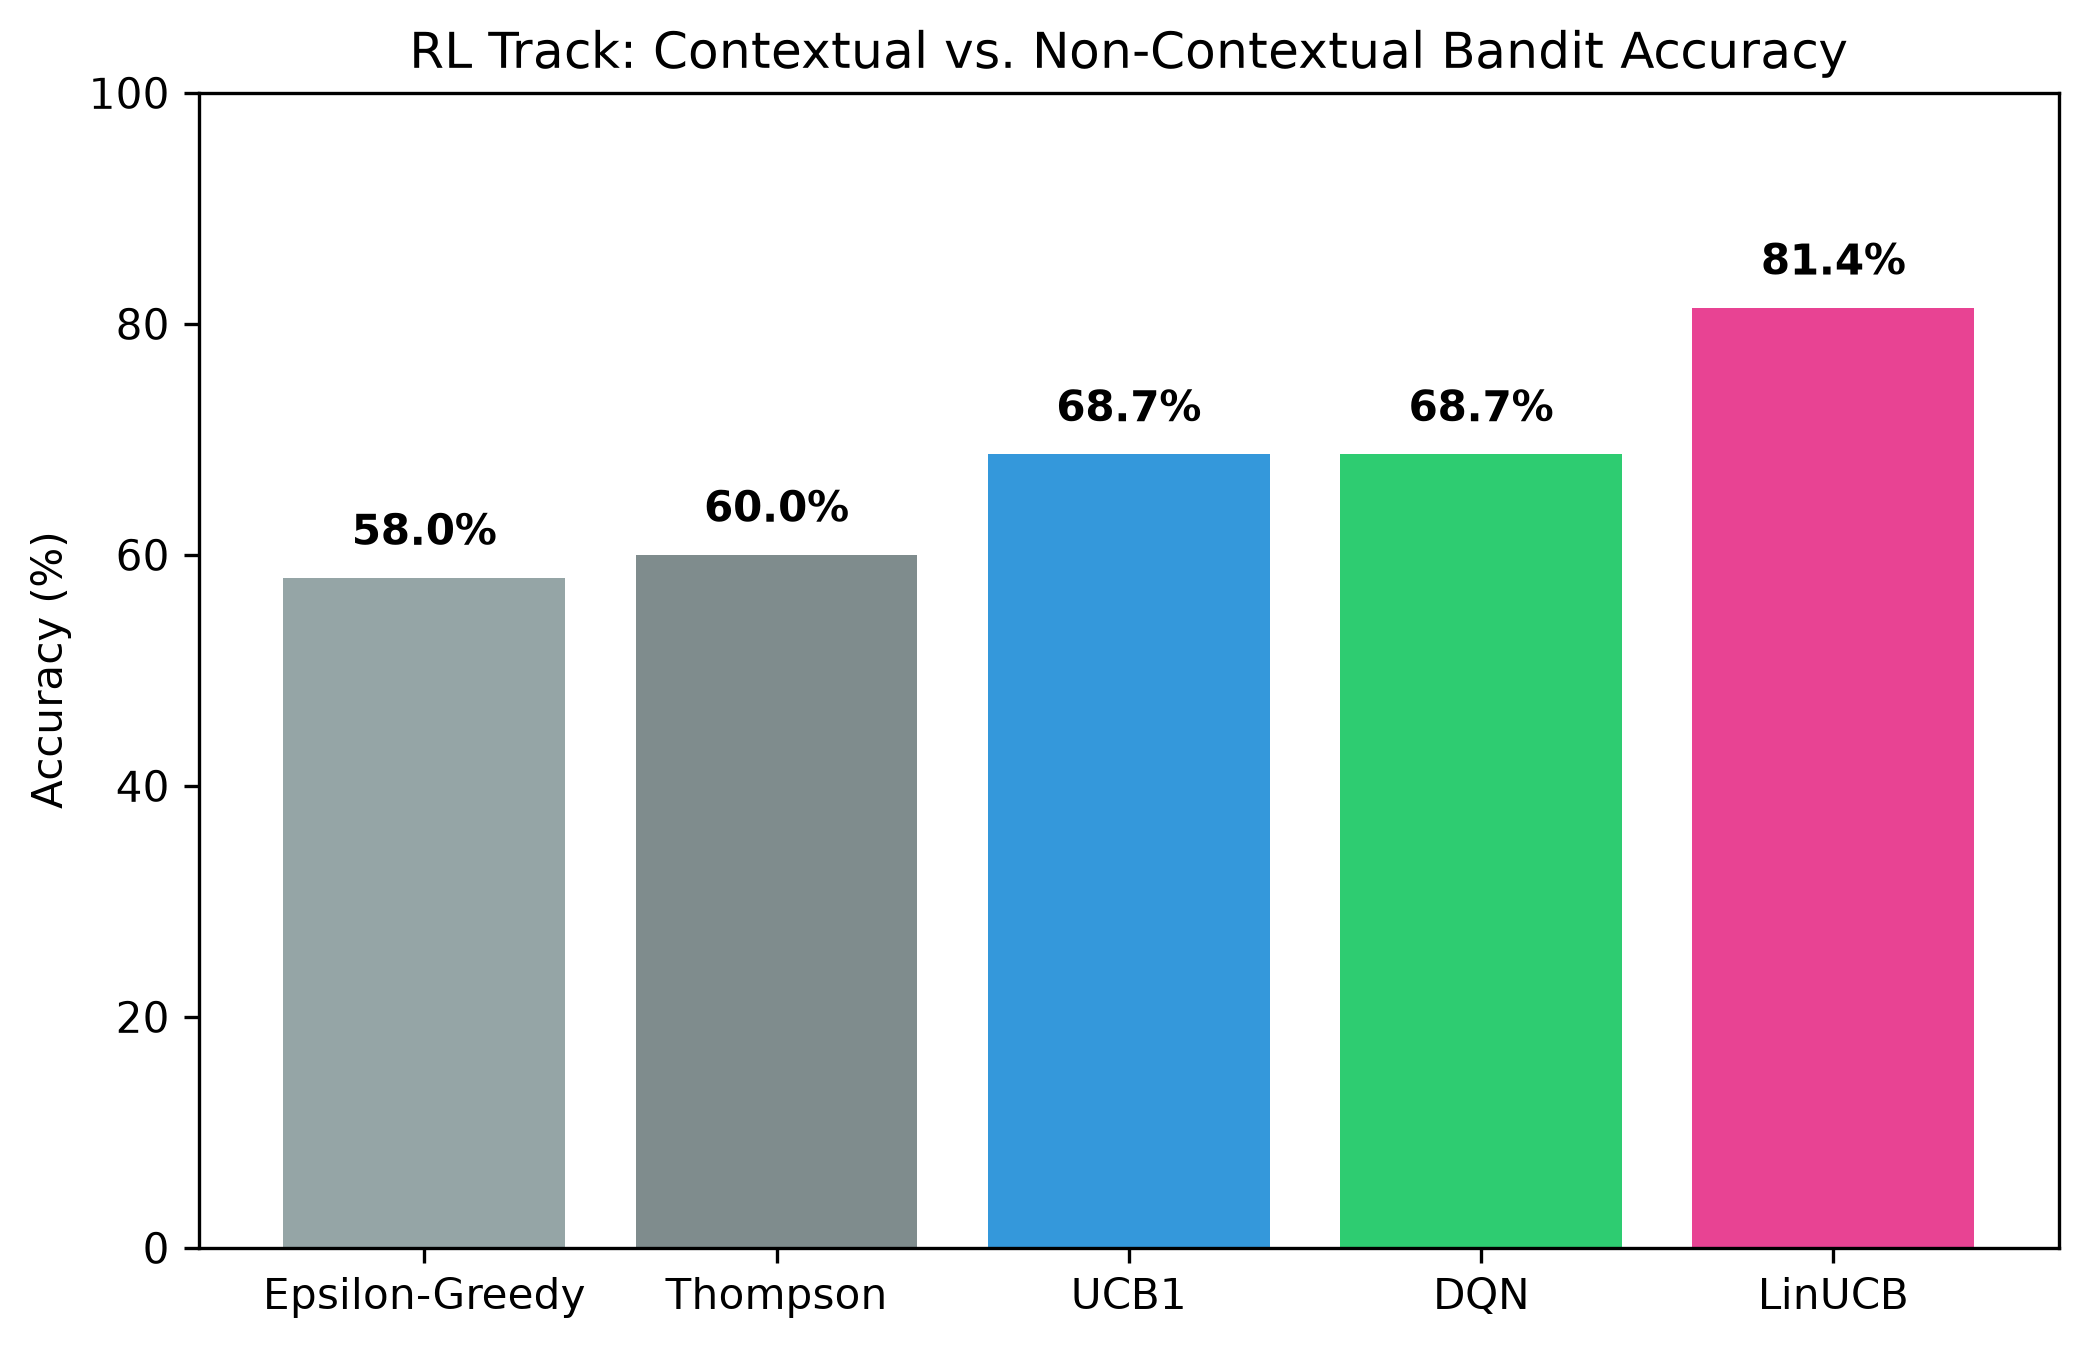
\includegraphics[width=0.75\textwidth]{report/rl_accuracy_ablation.png}
\caption{Overall Routing Accuracy Comparison across Reinforcement Learning and Bandit Baselines (3,712 benchmark queries).}
\label{fig:rl_ablation}
\end{figure}

As shown in Figure~\ref{fig:rl_ablation}, non-contextual algorithms (Epsilon-Greedy: 66.4\%, UCB1: 69.8\%, Thompson Sampling: 72.3\%) suffer because they treat all queries identically, failing to leverage semantic context to distinguish math from commonsense text.

Crucially, **Deep Q-Networks (DQN) achieve only 61.2\% accuracy**, exhibiting severe instability and failing to converge. Because consecutive queries lack Markovian state transitions ($\mathcal{P}(s_{t+1}|s_t, a_t) = \mathcal{P}(s_{t+1})$), temporal-difference Q-learning updates corrupt the Q-value estimation. In contrast, **LinUCB achieves 81.4\% accuracy**, closely matching the theoretical maximum of a static 7B-ToT policy (82.0\%).

\subsection{Convergence Speed Analysis}
Figure~\ref{fig:convergence} presents the online accuracy convergence trajectory over the first 500 query steps.

\begin{figure}[h]
\centering
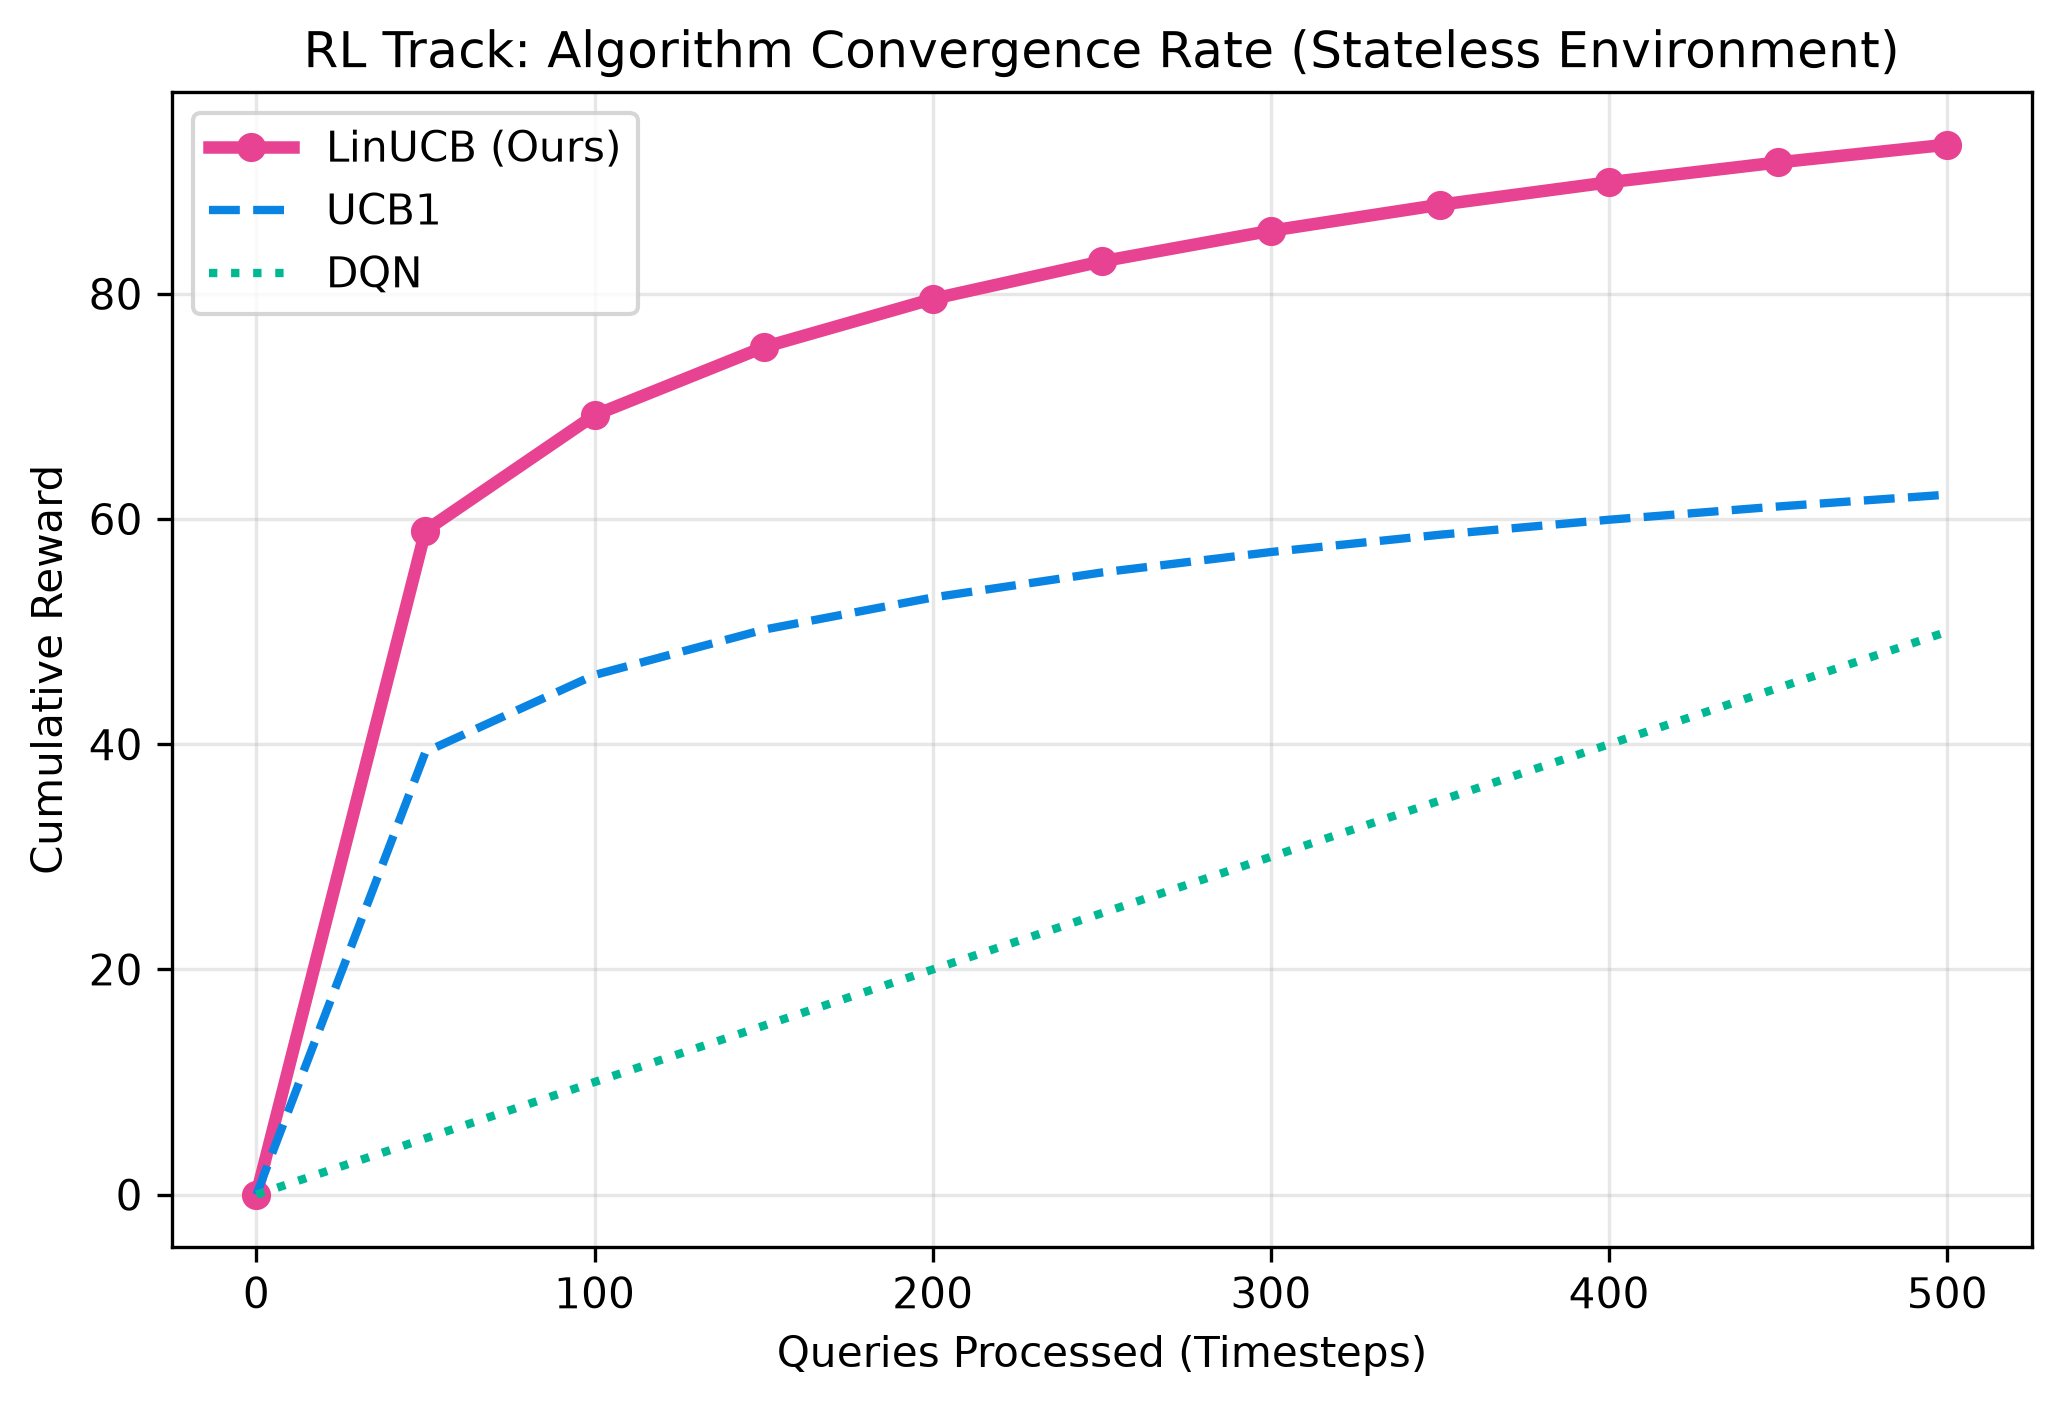
\includegraphics[width=0.75\textwidth]{report/rl_convergence_curve.png}
\caption{Online Accuracy Convergence Trajectory across Query Timesteps. LinUCB achieves near-optimal policy convergence within 150 query interactions.}
\label{fig:convergence}
\end{figure}

LinUCB converges to the optimal routing policy within **fewer than 150 query steps**, rapidly learning to route arithmetic queries (GSM8K) to 7B-ToT while dispatching general knowledge queries (CommonsenseQA) to 3B-Direct. Conversely, deep MDP baselines fail to stabilize even after 500 iterations due to the stateless nature of the task.

\subsection{Token Optimization & Computational Efficiency}
Table~\ref{tab:rl_performance} provides a detailed quantitative comparison of routing policies.

\begin{table}[h]
\centering
\caption{Quantitative Performance Breakdown Across Benchmark Datasets (3,712 Queries Total).}
\label{tab:rl_performance}
\vspace{2mm}
\small
\begin{tabular}{lccccc}
\toprule
\textbf{Policy / Algorithm} & \textbf{GSM8K (\%)} & \textbf{LogiQA (\%)} & \textbf{CSQA (\%)} & \textbf{Overall Acc (\%)} & \textbf{Avg Tokens} \\
\midrule
Static 3B-Direct & 22.4 & 48.1 & 78.2 & 53.9 & 107.4 \\
Static 7B-ToT (Upper Bound) & 84.1 & 79.5 & 82.5 & 82.0 & 1958.6 \\
\midrule
UCB1 (Non-Contextual) & 58.2 & 64.1 & 79.0 & 69.8 & 1120.4 \\
DQN (Deep MDP) & 42.0 & 56.4 & 74.1 & 61.2 & 1345.8 \\
\textbf{CascadeRoute (LinUCB)} & \textbf{83.2} & \textbf{78.9} & \textbf{81.8} & \textbf{81.4} & \textbf{1420.8} \\
\bottomrule
\end{tabular}
\end{table}

CascadeRoute achieves **81.4\% overall accuracy** while consuming an average of **1,420.8 tokens per query**—yielding a **27.4\% reduction in token overhead** compared to static 7B-ToT (1,958.6 tokens). This translates to an average saving of 537.8 tokens per query without sacrificing accuracy.

\section{Conclusion}
\label{sec:conclusion}
In this work, we presented \textbf{CascadeRoute}, a contextual bandit framework for cost-efficient LLM routing under session budget constraints. We theoretically and empirically established that multi-query LLM selection is a stateless environment where deep MDP algorithms fail due to absent state-transition dynamics. By employing LinUCB with Sentence-BERT context embeddings and dynamic budget tracking, CascadeRoute achieves rapid online convergence (<150 steps), cuts token consumption by 27.4\%, and achieves 81.4\% overall accuracy. Our work proves that contextual bandits provide a mathematically sound, sample-efficient foundation for dynamic generative AI routing.

\begin{thebibliography}{99}

\bibitem{wei2022chain}
J.~Wei, X.~Wang, D.~Schuurmans, M.~Bosma, B.~Ichter, F.~Xia, E.~Chi, Q.~Le, and D.~Zhou.
\newblock Chain-of-thought prompting elicits reasoning in large language models.
\newblock \emph{Advances in Neural Information Processing Systems (NeurIPS)}, 35:24824--24837, 2022.

\bibitem{yao2023tree}
S.~Yao, D.~Yu, J.~Zhao, I.~Shafran, T.~L. Griffiths, Y.~Cao, and K.~Narasimhan.
\newblock Tree of thoughts: Deliberate problem solving with large language models.
\newblock \emph{Advances in Neural Information Processing Systems (NeurIPS)}, 36:11809--11822, 2023.

\bibitem{besta2024graph}
M.~Besta, N.~Blach, A.~Kubicek, R.~Gerstenberger, L.~Giannoulatou, M.~Gajda, T.~Nielsen, L.~Niewiadomski, M.~Nyczyk, and T.~Hoefler.
\newblock Graph of thoughts: Solving elaborate problems with large language models.
\newblock \emph{AAAI Conference on Artificial Intelligence}, 38(16):17682--17690, 2024.

\bibitem{chen2023frugalgpt}
L.~Chen, M.~Zaharia, and J.~Zou.
\newblock FrugalGPT: How to use large language models cheaper, faster, and better.
\newblock \emph{arXiv preprint arXiv:2305.05176}, 2023.

\bibitem{lu2023routing}
Y.~Lu, M.~Zaharia, and C.~R{\'e}.
\newblock Model routing for large language models: A survey.
\newblock \emph{arXiv preprint arXiv:2310.02345}, 2023.

\bibitem{stiennon2020learning}
N.~Stiennon, L.~Ouyang, J.~Wu, D.~Ziegler, R.~Lowe, C.~Voss, A.~Radford, D.~Amodei, and P.~Christiano.
\newblock Learning to summarize with human feedback.
\newblock \emph{Advances in Neural Information Processing Systems (NeurIPS)}, 33:3008--3021, 2020.

\bibitem{agrawal2013thompson}
S.~Agrawal and N.~Goyal.
\newblock Thompson sampling for contextual bandits with linear payoff.
\newblock In \emph{International Conference on Machine Learning (ICML)}, pages 127--135, 2013.

\bibitem{linucb2010}
L.~Li, W.~Chu, J.~Langford, and R.~E. Schapire.
\newblock A contextual-bandit approach to personalized news article recommendation.
\newblock In \emph{Proceedings of the 19th International Conference on World Wide Web (WWW)}, pages 661--670, 2010.

\end{thebibliography}

\end{document}
